\section{Rate-Distortion Theory} \label{sec:rdt}
Il primo teorema di Shannon si riferisce a codifica senza perdita e a sorgenti discrete. Quando si ha a che fare
con la codifica lossless, non ci si deve preoccupare di come avverrà la ricostruzione dell’informazione dopo
la decodifica perché sappiamo che il processo è completamente reversibile, quindi la ricostruzione in
decodifica è identica all’originale. Tuttavia, Shannon ci dice che se vogliamo preservare tutta l’informazione
della sorgente, la capacità di compressione ha un limite fondamentale che è dato dall’entropia. \\
In alcuni casi ed applicazioni la compressione lossless può andare bene, ma in altri può essere necessario aumentare il tasso di compressione accettando un certo livello di perdita di informazione, ovvero facendo una codifica \textit{lossy}. Inoltre si deve tenere in considerazione che quando la sorgente informativa è analogica per
trasformarla in numerica si effettua \textit{sempre} una codifica di sorgente lossy.

Se nella codifica lossless l’unica metrica di interesse è il \textit{rate di generazione} $R$, ovvero il \textbf{numero di bit per simbolo necessari a rappresentare la sorgente}, nella codifica lossy questo non basta, infatti se così fosse, la migliore forma di codifica sarebbe buttare via tutti i dati. \\
Quando si ha codifica lossy ci interessa quindi il rate ma anche la perdita di informazione, ovvero una misura della differenza tra l’informazione originaria e quella ricostruita. La perdita dell’informazione viene denominata \textbf{distorsione}.

La \textit{distorsione} $D$ è tanto maggiore tanto pi\`u i dati ricostruiti, a valle della compressione, distano in qualità dai dati originali. Il concetto di qualità (distorsione accettabile) non è un concetto assoluto, ma dipende necessariamente dall’\textit{applicazione} dei dati, e cioè dall’impiego che si fa dei dati ricostruiti e da chi ne usufruisce. \\
Si hanno diversi modi di misurare la distorsione e la qualità di un segnale ricostruito e diversi livelli di distorsione accettabili. In ogni caso, comunque sia definita la misura della distorsione, ci\`o che si desidera è trovare una tecnica di codifica che per ogni fissato livello di distorsione $D$ codifichi la sorgente al tasso $R$ più piccolo possibile (o, al contrario, che per ogni fissato tasso di codifica $R$ comporti la minima distorsione $D$).

La Rate-Distortion Theory è il ramo della teoria dell’informazione che descrive il \textit{trade-off} tra il rate di trasmissione (bit/simbolo usati per la codifica) e la corrispondente distorsione e fornisce i limiti per la compressione con perdita. Si sottolinea come questa sia essenziale per sorgenti continue per le quali non \`e possibile avere una codifica lossless. \\
La Rate-Distortion Theory si occupa quindi di trovare le prestazioni limite teoriche, in termini di funzioni $R(D)$ e $D(R)$ per assegnate sorgenti e misure di distorsione.
A livello pratico si vuole
\begin{itemize}
    \item Definire un modo per misurare la distorsione $D$.
    \item Determinare il rate minimo (massima compressione) $R$ a cui si può lavorare ammettendo una certa distorsione o, equivalentemente, la distorsione minima che si ha lavorando con un certo rate.
\end{itemize}
Come nel caso della codifica lossless la teoria dell’informazione fornisce dei limiti teorici che poi servono per
la progettazione delle tecniche di codifica. Tuttavia in caso di codifica con perdita, anche per sorgenti
piuttosto semplici, esistono pochi risultati in forma chiusa della rate-distortion theory, e si dovr\`a quindi ricorrere ad approssimazioni. Inoltre, anche quando le curve limite sono note, i metodi di codifica esistenti forniscono prestazioni lontane da quelle ottime, soprattutto a causa dei vincoli di memoria e complessità computazionale ai quali si deve sottostare.
\begin{figure}[H]
    \centering
    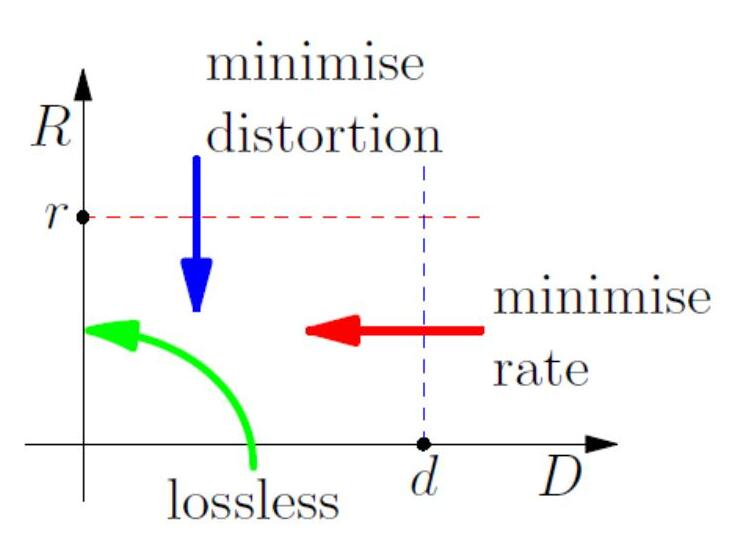
\includegraphics[scale=0.2]{img/rdt.jpg}
    \caption{Obiettivo della RDT.}
    \label{fig:rtd}
\end{figure}

\subsection{Distorsione}
Dato che la valutazione della qualità della codifica dipende dall’uso che si deve fare dei dati codificati non è possibile definire un metodo di misura universalmente valido. Si deve scegliere allora il metodo che di volta in volta risulta più adatto all’applicazione. Sia $x \in X$ un elemento dell'alfabeto della sorgente e sia $\hat{x} \in \hat{X}$ l'elemento stesso ricostruito dal ricevitore. Dovendo quantificare la distorsione dovremo avere che questa sia, in qualche modo, funzione di una distanza $d(\cdot, \cdot)$ tra i due oggetti. Vediamo due metriche di distanza per variabili aleatorie:
\begin{enumerate}
    \item Nel caso di sorgenti binarie una misura comunemente usata è la \textit{Distanza di Hamming:} \begin{equation}
        d(x, \hat{x}) = x \oplus \hat{x} \coloneqq \begin{cases}
        0, & \text{se } x = \hat{x} \\
        1, & \text{se } x \neq \hat{x}
        \end{cases}
    \end{equation}
    \item Nel caso di sorgenti continue il modo più naturale per vedere la fedeltà della ricostruzione è fare la differenza tra i valori iniziali e quelli ricostruiti. Il più popolare è l’\textit{errore quadratico} (SE):
    \begin{equation*}
        d(x, \hat{x}) = (x - \hat{x})^2
    \end{equation*}
\end{enumerate}
Ovviamente può essere definita anche in altro modo, ad esempio come la differenza assoluta tra due campioni. In
generale, la cosa migliore di tutti sarebbe tener conto dell’effetto finale della distorsione, ovvero come questa
viene percepita: tale valutazione non è per\`o una misura oggettiva, ma dipendente dal contesto e quindi per poterla effettivamente quantificare si deve ricorrere a misure come l’MSE che non sono perfette ma semplici e oggettive. Ad esempio nel caso della trasmissione di segnali vocali anche se l'MSE è alto si può avere una buona percezione, ovvero che la distorsione percepita è bassa.
\defn{\textit{Distorsione:}} La distorsione $D$ \`e definita come
\begin{equation}
    D = \mathbb{E} [ d(X, \hat{X})]
\end{equation}
dove la media viene fatta su tutti gli elementi dell'alfabeto $X$ e su tutti i possibili simboli ricostruiti dell'alfabeto $\hat{X}$, quindi sulla distribuzione congiunta $p(x, \hat{x})$.\\
Nei due casi precedenti quindi si ha
\begin{itemize}
    \item La probabilit\`a di ricostruire in modo sbagliato $D = \mathbb{E} [X \oplus \hat{X}] \coloneqq P_e$
    \item Il Mean Squared Error (MSE) dato da $D = \mathbb{E} [(X - \hat{X})^2]$
\end{itemize}
La distorsione con la distanza di Hamming prende il nome di \textit{probability of a reconstruction error} dal momento che $\mathbb{E}[X \oplus \hat{X}] = 0 \times Pr\{x=\hat{x}\} + 1 \times Pr\{x \neq \hat{x}\} = P_e$.\\
Estendendo alle sequenze di simboli $x^n, \hat{x}^n$ si ha
\begin{equation}
    d(x^n, \hat{x}^n) = \frac{1}{n} \sum_{i=1}^n d(x_i, \hat{x}_i)
\end{equation}
che, nel caso di sorgenti stazionarie (\textit{i.i.d}), porta allo stesso valor medio
\begin{equation}
    D = \mathbb{E} [d(X^n, \hat{X}^n) = \mathbb{E}[d(X, \hat{X})]
\end{equation}
Si pu\`o definire anche un'altra importante grandezza: il rapporto segnalre-rumore (\textbf{SNR}). Il rapporto segnale-rumore è un numero puro o adimensionale, dato dal rapporto fra due grandezze omogenee, che esprime quanto il segnale sia \textit{più potente} del rumore nel sistema considerato. È formalmente espresso dalla relazione: 
\begin{equation}
    SNR = \frac{\sigma_x^2}{\sigma_d^2}
\end{equation}
dove $\sigma_x^2$ rappresenta la potenza del segnale utile e $\sigma_d^2$ la potenza totale del rumore presente nel sistema (dato dalla distorsione). Queste vengono solitamente espresse in $Watt$ o $dBm$. Più basso è l'SNR, più sarà difficoltosa la decodifica del segnale ovvero più alta sarà la probabilità di errore.

\subsection{Funzione di Rate-Distortion}
Data una distribuzione statistica della sorgente e una misura della distorsione $D$, la domanda a cui si prova
a rispondere è \emph{quale è la minima distorsione $D$ ottenibile quando viene fissata una velocità di trasmissione $R$?} La funzione di Rate-Distortion $R(D)$ fornisce il numero minimo di bit (cio\`e il rate minimo $R$) che si può usare per rappresentare una sorgente e che garantisce un errore di ricostruzione
\begin{equation}
    \mathbb{E} [d(X, \hat{X})] \leq D
\end{equation}
Il caso $D = 0$ significa che non viene accettata distorisione da cui $R(0)$ nel caso di sorgenti discrete coincide con l'entropia della sorgente $H(X)$ e, nel caso di sorgenti continue, $R(0) = \infty$. \\
$R(D)$ è una funzione monotona decrescente di $D$. Equivalentemente potremmo anche determinare l'inversa $D(R)$, rispondendo alla domanda \emph{qual è la velocità minima (numero minimo di bit per
la rappresentazione) che si può avere per garantire una data distorsione?} In questo caso la funzione inversa
$D(R)$ (Distortion-Rate) fornisce il livello di distorsione del segnale riscostruito fissato il massimo numero di bit che si possono spendere per la rappresentazione.
\begin{figure}[H]
    \centering
    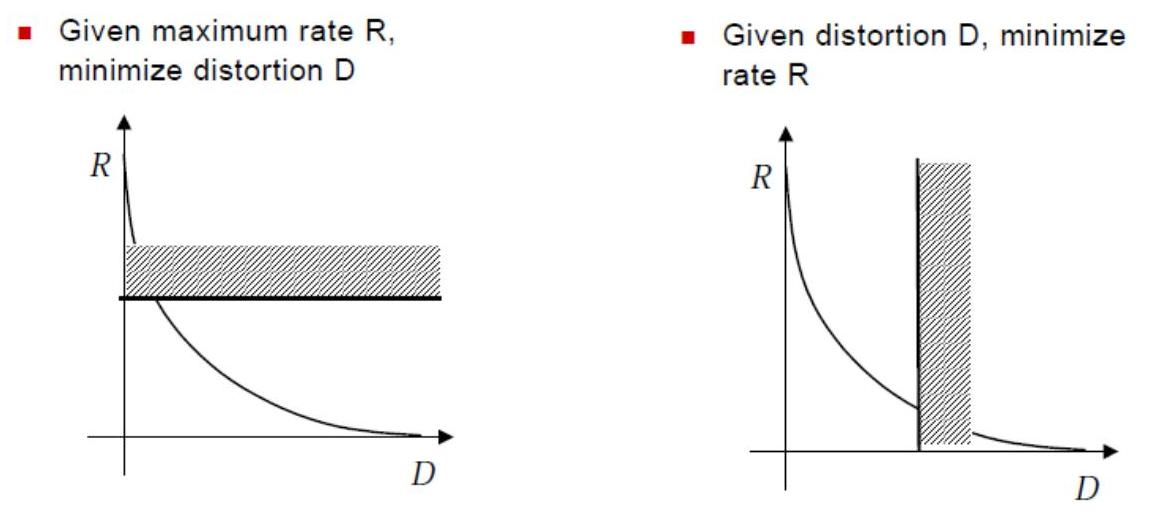
\includegraphics[scale=0.2]{img/rdf.jpg}
    %\caption{Rate-Distorsion}
    \label{fig:rdf}
\end{figure}
\defn{\textit{Raggiungibilit\`a:}} Una coppia $(R,D)$ si dice raggiungibile se esiste una codifica a rate $R$ tale che
\begin{equation}
    \lim_{n \to \infty} \frac{1}{n} \sum_{i=1}^n d(x_i, \hat{x}_i) \leq D
\end{equation}
La \textbf{regione di rate-distortion} $\mathcal{R}$ rappresenta l’insieme dei punti $(R,D)$ raggiungibili e la funzione di rate distortion è l’estremo inferiore dei rate $R$ tali che $(R,D) \in \mathcal{R}$ per ciascun valore di $D$ fissato. \\
La funzione di rate-distortion $R(D)$ è quindi il \textit{lower-bound del rate di trasmissione per un fissato valore di distorsione $D$:} Se $R > R(D)$ allora esiste una sequenza di codici con una distorsione media che si avvicina a $D$, altrimenti se il rate \`e nella zona inferiore, tali codici non esistono.
\begin{figure}[H]
    \centering
    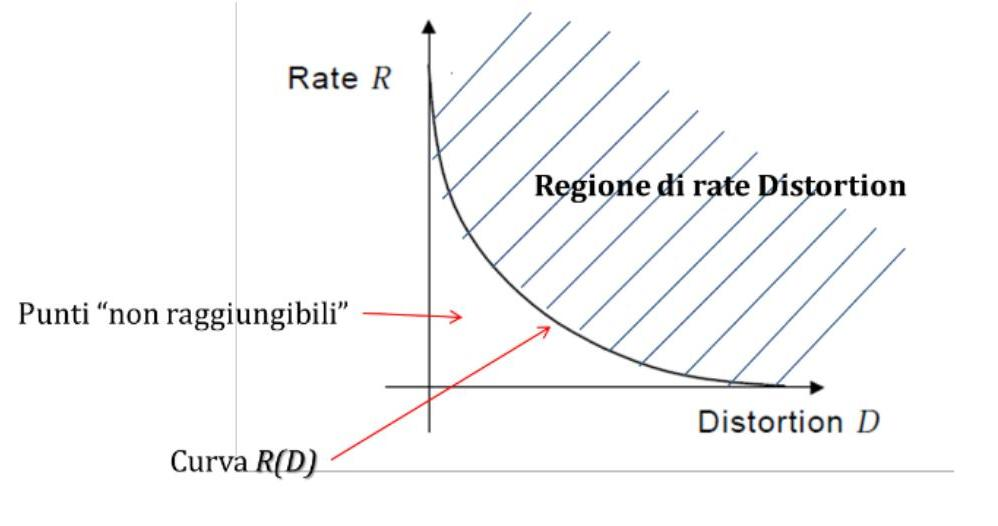
\includegraphics[scale=0.3]{img/rdc.jpg}
    \caption{Regione di rate distortion.}
    \label{fig:rdc}
\end{figure}
Il principale Teorema della Rate Distortion Theory \`e dovuto a Shannon (1956) ed \`e noto come \textit{Lossy Coding Theorem} (Teorema della Codifica con Perdita):

\textbf{Teorema}: Sia $(X,\hat{X}) \sim p(x, \hat{x})$ con allora la funzione $R(D)$ per la sorgente\footnote{La stessa definizione vale nel caso continuo utilizzando le funzioni densità di probabilità.} $X$ con simboli \textit{i.i.d.} e funzione di distanza $d(x, \hat{x})$ \`e data da
\begin{align*}
    R(D) = &\min_{p(x|\hat{x})} I(X; \hat{X}) \\
    &\text{s.t. } \mathbb{E}[d(X, \hat{X})] \leq D
\end{align*}
Fissata un valore di distorsione $D$, il minimo rate $R$ possibile si trova minimizzando l’informazione muta, tra tutte le coppie $(x, \hat{x})$ (e quindi tra tutte le possibili codifiche $\hat{x} = C(x)$) che soddisfano $D$. Si noti come il vero grado di libert\`a nella minimizzazione sia la distribuzione condizionata $p(\hat{x}|x)$, derivante dal fatto che la minimizzazione avvenga su $p(x, \hat{x}) = p(\hat{x}|x)p(x)$ in cui $p(x)$ dipende dalla sorgente mentre $p(\hat{x}|x)$ descrive la codifica ed \`e quello che ci permette di minimizzare $I(X; \hat{X})$.\\
L’informazione mutua tra due sorgenti ci dice quanto di una sorgente è contenuto nell’altra, in questo caso
quanto dell’informazione originaria è contenuta in quella ricostruita, dopo la codifica/decodifica con perdita. 

Ricapitolando: più la codifica comprime (più si riducono i bit di rappresentazione $R$) e più si perde informazione. Si avrà quindi sempre meno informazione di $X$ contenuta in $\hat{X}$ e $I(X; \hat{X})$ diminuir\`a. Quest'ultima per\`o può diminuire solo fino al limite in cui garantisce il vincolo sulla distorsione $D$, restringendo quindi l'insieme di coppie ($X, \hat{X})$ ammissibili.

Se si ha una sorgente continua  e la si quantizza questa  è  una  forma  di  codifica  con  perdita: fissata  la  massima distorsione che si vuole avere (che corrisponde all’errore di quantizzazione) si fissano i livelli di quantizzazione, e quindi i bit di rappresentazione, e quindi il rate.

\begin{mybox}{green}{\textit{\textbf{Esempio 1} : \textbf{R(D) per una sorgente gaussiana. }}}
Sia $X \sim \mathcal{N}(0, \sigma^2)$. Per questo genere di sorgenti \`e ragionevole adottare la distanza a errore quadratico. La funzione di rate distortion $R(D)$ \`e data da
\begin{equation*}
    R(D) = \begin{cases}
    \frac{1}{2} \log \frac{\sigma^2}{D} & \text{se } 0 \leq D \leq \sigma^2 \\
    0 & \text{se } D > \sigma^2
    \end{cases}
\end{equation*}
Dal momento che la funzione \`e invertibile in $[0, \sigma^2]$ si ha
\begin{equation*}
    D(R) = \sigma^2 2^{-2R}
\end{equation*}
infatti 
\begin{equation*}
    2^{R(D)} = 2^{\frac{1}{2} \log (\frac{\sigma^2}{D})} = 2^{\log \frac{\sigma}{\sqrt{D}}} = \frac{\sigma}{\sqrt{D}} \implies \sqrt{D} = \frac{\sigma}{2^R} \implies D = \sigma^2 2^{-2R}
\end{equation*}
Inoltre il $SNR$ associato alla distorsione \`e dato da
\begin{equation*}
    SNR = \frac{\sigma^2}{D} = 2^{2R}
\end{equation*}
da cui
\begin{equation*}
    SNR_{db} \approx 6R
\end{equation*}
ovvero, se si aumenta di 1 bit il rate (si rappresenta con un bit in più i simboli della sorgente in media) la
distorsione si riduce di $\frac{1}{2^2}$ cio\`e di circa $6 db$.
\end{mybox}

\subsection{Rate-Distortion Bounds}
Spesso non è possibile trovare la funzione di Rate-Distortion per sorgenti con distribuzione qualsiasi. In questi casi è quindi utile avere dei limiti (superiori ed inferiori) che forniscono comunque un range di valori “raggiungibili”, che quindi possono essere presi a riferimento per la progettazione e per valutare margini di miglioramento. \emph{In questo modo la funzione di rate-distortion gioca lo stesso ruolo per la compressione con perdita dell’entropia nel caso di quella senza perdita.}

Si può dimostrare che per una generica sorgente continua con pdf $f_X(x)$ a media nulla e varianza $\sigma^2$, se la distorsione \`e misurata come un MSE, allora vale
\begin{equation}
    h(x) - \frac{1}{2} \log (2\pi e D) \leq R(D) \leq \frac{1}{2} \log \frac{\sigma^2}{D}
\end{equation}
Per una variabile aleatoria gaussiana questi due bound coincidono.
\subsection{Quantizzazione}
\textit{Quando la sorgente d’informazione è continua, il processo di acquisizione dei dati è un processo con perdita di informazione:} l’informazione deve essere discretizzata attraverso il del campionamento e i valori continui devono essere rappresentati con una stringa \textit{finita} di simboli binari. La perdita di informazione dovuta alla quantizzazione è inevitabile quando si passa da sorgenti continue a sistemi digitali, però è una perdita controllata, e può essere usata per diminuire la quantità di dati da gestire (ovvero diminuire il rate del segnale).

\begin{center}
\emph{“The question is: can we assign a definite rate to a continuous source when we require only a certain fidelity of recovery, measured in a suitable way?”}\\
Shannon, A Mathematical Theory of Communication.
\end{center}

Per la progettazione di un quantizzatore quindi la questione è \textit{come trovare la migliore possibile
rappresentazione} di una sorgente continua dato un certo rate di trasmissione $R$. Esistono vari tipi di
quantizzatori e ciascuno porta ad un certo valore di $D$.\\
In generale la quantizzazione è un processo molto semplice: si rappresentano tutti i possibili valori assunti
dai simboli sorgente, con un ben più ristretto set di valori.
\begin{figure}[H]
    \centering
    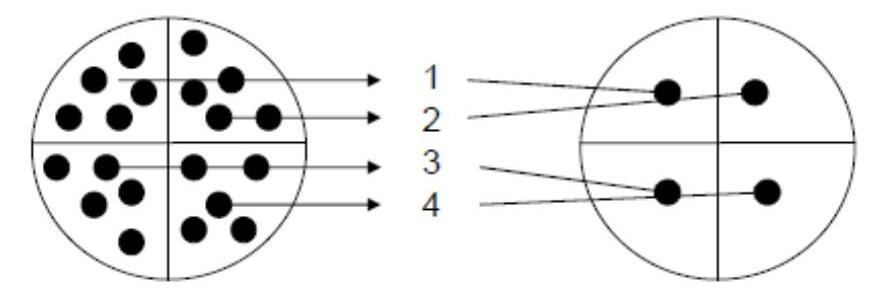
\includegraphics[scale=0.2]{img/quant.jpg}
    \caption{Perdita della iniettivi\`a.}
    \label{fig:quant}
\end{figure}
Il quantizzatore divide il range di valori che una sorgente genera in un numero finito di intervalli ciascuno dei quali è rappresentato da un \textit{valore di riferimento} e poi da una parola di codice (binaria): infiniti valori possono cadere nello stesso intervallo e quindi il processo è irreversibile. Conoscere la parola di codice permette di conoscere solo l’intervallo di appartenenza e non pi\`u quale degli infiniti valori iniziali fosse quello corretto. La costruzione degli intervalli di valori e di come questi sono rappresentati sono parte della progettazione del codificatore di sorgente.\\
È necessario quindi capire come dividere il range di ingresso in intervalli e come assegnare i codici binari a ciascun intervallo per avere un rate e/o una distorsione desiderati\footnote{Come detto prima un criterio può essere quello di prendere come misura di distorsione l’errore quadratico medio.}.\\
Supponiamo che la nostra sorgente sia caratterizzata da una pdf $f_X(x)$ e che la dinamica di ingresso venga
divisa in $m$ intervalli $[x_i, x_{i+1}), i=1,\dots, m$, ciascuno rappresentato dal valore di riferimento $\hat{x}_i$.
\begin{figure}[H]
    \centering
    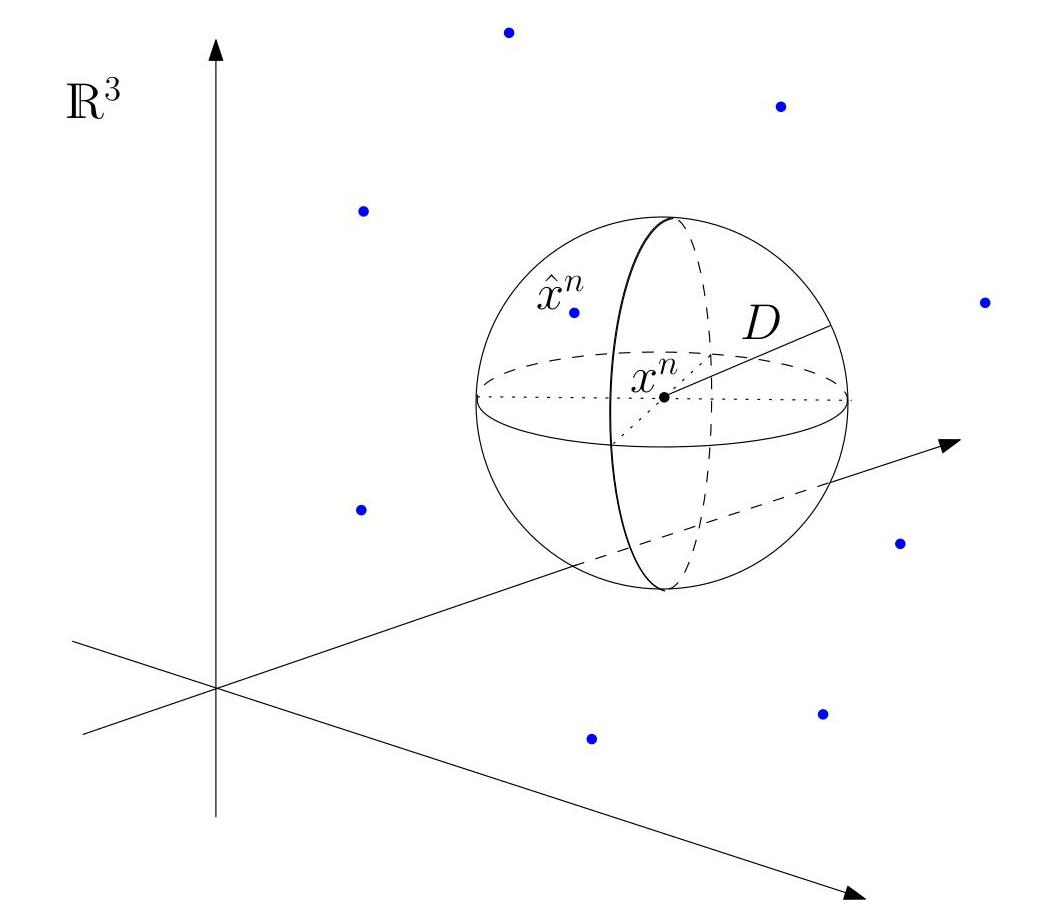
\includegraphics[scale=0.23]{img/sphere.jpg}
    \caption{Rappresentazione tridimensionale della regione di quantizzazione.}
    \label{fig:sphere}
\end{figure}
L'operazione di \textbf{quantizzazione} \`e data da una certa funzione $Q(\cdot)$
\begin{equation}
    \hat{x}_i = Q(x), \hspace{15pt} \text{se } x_i \leq x \leq x_{i+1}
\end{equation}
L'MSE \`e dato invece da
\begin{equation}
    D = \mathbb{E}[(x - Q(x))^2] =  \int_{-\infty}^{\infty} \Big ( x - Q(x) \Big )^2 f_X(x) dx = \sum_{i=1}^m \int_{x_i}^{x_{i+1}} (x - \hat{x}_i) f_X(x) dx
\end{equation}
La differenza tra il campione originario e quello quantizzato prende il nome di \textit{distorsione di quantizzazione} o \textit{rumore di quantizzazione}.

Ciascuno di questi intervalli dovr\`a essere poi codificato: se si usano per la codifica parole di codice della stessa lunghezza $l$ ($l = \lceil \log m \rceil$) la progettazione del quantizzatore, dati $f_X(x)$ e $m$, si riduce a determinare gli intervalli $x_i$ e i valori $\hat{x}_i$ che li rappresentano. Si potrebbero tuttavia utilizzare parole di lunghezza diversa $l_i$ (come ad esempio nella codifica di Huffman) e allora la scelta degli intervalli \textit{influenza anche il rate $R$ della sorgente}:
\begin{equation}
    R = \sum_{i=1}^m l_i p(\hat{x}_i) = \sum_{i=1}^m l_i \int_{x_i}^{x_{i+1}} f_X(x) dx
\end{equation}
Possiamo concludere che:
\begin{itemize}
    \item La distorsione $D$ dipende da come vengono scelti gli intervalli e dai \textit{valori} $\hat{x}_i$ scelti per rappresentarli.
    \item Il rate $R$ dipende da come vengono scelti gli intervalli e dai \textit{codici} usati per rappresentarli.
\end{itemize}
Si ha quindi che i problemi di trovare le migliori partizioni, rappresentazioni e codifica sono legati tra loro. \\
Quindi, ricapitolando: \\
Dato un limite di distorsione $D^*$ (massimo tollerato) si devono determinare gli intervalli di quantizzazione $[x_i, x_{i+1})$ e i valori che li rappresentano $\hat{x}_i$ in modo che soddisfino:
\begin{equation}
    \begin{cases}
    D \leq D^* \\
    R = \sum_{i} l_i p(\hat{x}_i) = \sum_i l_i \int_{x_i}^{x_{i+1}} f_X(x) dx
    \end{cases}
\end{equation}
oppure, equivalentemente, dato un limite massimo di rate $R^*$ si devono trovare i valori degli intervalli di quantizzazione $[x_i, x_{i+1})$ e le parole di codice tali che soddisfino:
\begin{equation}
    \begin{cases}
    R \leq R^* \\
    D = \int_{-\infty}^{\infty} \Big ( x - Q(x) \Big )^2 f_X(x) dx = \sum_{i}^m \int_{x_i}^{x_{i+1}} (x - \hat{x}_i) f_X(x) dx
    \end{cases}
\end{equation}
\subsubsection{Quantizzazione scalare}
Un quantizzatore scalare, associa ad ogni valore continuo della sorgente un valore $\hat{x}_i$ appartenente ad un set discreto di $m$ valori ciascuno dei quali rappresenta una particolare porzione dell’asse dei numeri reali $[x_i, x_{i+1})$ e $\hat{x}_i$ \`e un valore interno a tale intervallo. Un quantizzatore di largo impiego è quello \textbf{uniforme}, in cui tutti gli intervalli di
quantizzazione sono uguali. È completamente caratterizzato dall'ampiezza $\Delta$ dell'intervallo di quantizzazione (lo step di quantizzazione) e dal numero di livelli $m=2^R$.\\
Se la sorgente $X$ \`e uniforme sull'intervallo $[-A, A]$ si pu\`o pensare che la quantizzazione uniforme sia la scelta pi\`u appropriata: fissato $m$ vogliamo trovare il valore $\Delta$ che minimizza la distorsione $D$, ovvero l'errore di quantizzazione. Essendo la distribuzione uniforme si vede facilmente che 
\begin{equation}
    \Delta = \frac{2A}{m}
\end{equation}
e che l'errore di quantizzazione $e_q \coloneqq |x_i - \hat{x}_i|$ \`e distribuito uniformemente sull intervallo $[-\frac{\Delta}{2}, \frac{\Delta}{2}]$. La distorsione (MSE) in questo modo diventa
\begin{align*}
    D &= \mathbb{E} [ (X - \hat{X})^2] = \int_{-\infty}^{\infty} \Big ( x - Q(x) \Big )^2 f_X(x)dx = \\
    &= \sum_{i=1}^m \int_{x_i}^{x_{i+1}} (x - \hat{x}_i)^2 f_X(x) dx = \\
    &= \sum_{i=1}^m \frac{1}{2A} \int_{x_i}^{x_{i+1}} (x - \hat{x}_i)^2 dx = \frac{m}{2A} \int_{-\frac{\Delta}{2}}^{\frac{\Delta}{2}} x^2 dx = \\
    &= \frac{1}{\Delta} \int_{-\frac{\Delta}{2}}^{\frac{\Delta}{2}} x^2 dx = \frac{\Delta^2}{12}
\end{align*}
Ricordando che la varianza di una sorgente uniformemente distribuita su $[-A, A]$ \`e data da $A^2/3$ si ha che
\begin{equation}
    SNR = \frac{A^2/3}{\Delta^2/12} = \frac{12A^2}{3\Delta^2} = \frac{4A^2}{\Delta^2} = m^2 = 2^{2R} \approx 6R \hspace{2pt} db
\end{equation}

Non sempre la quantizzazione uniforme da buoni risultati, infatti l’errore di quantizzazione che si compie
dipende anche dalla statistica della sorgente. Il quantizzatore uniforme si comporta in maniera ottima
(minima potenza del rumore di quantizzazione) \textit{solo se le ampiezze dei campioni del segnale sono caratterizzate da una distribuzione uniforme}. Se la sorgente non è uniformemente distribuita ci sono range di valori in cui è più probabile avere un campione della sorgente ed è quindi meglio aumentare la densità dei livelli di quantizzazione nelle zone più popolate, in modo da avere una maggiore «accuratezza» dove si hanno più campioni, diminuendo di conseguenza la distorsione.\\
Quest'ultima può essere quindi ridotta scegliendo gli intervalli di quantizzazione in funzione delle statistiche
di $X$ (tenendo conto della pdf della sorgente), il che ci porta a una \textbf{quantizzazione non uniforme}: \textit{assegnare intervalli più stretti per le ampiezze più frequenti e intervalli di dimensioni crescenti per le ampiezze meno frequenti.} Facendo così si presta quindi più attenzione nella quantizzazione di valori che si presentano con maggiore probabilità diminuendo così l'errore di quantizzazione. \\
L'obiettivo della quantizzazione non uniforme è quindi trovare l’ampiezza degli intervalli ed i valori che li rappresentano tali che minimizzino la distorsione, fissato $m$.

\begin{figure}[H]
    \centering
    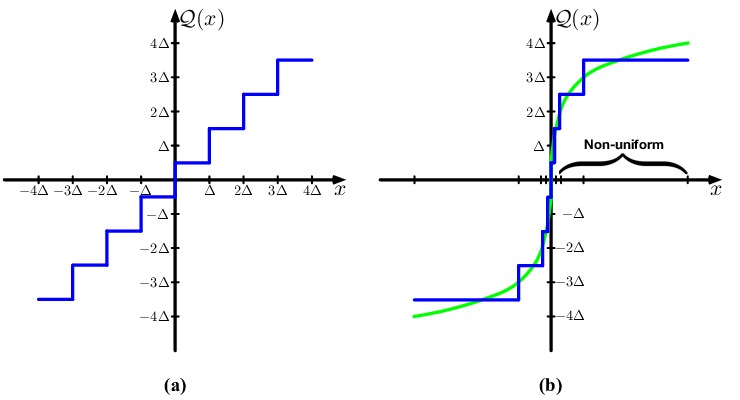
\includegraphics[scale=0.3]{img/uniform.png}
    \caption{Quantizzazione uniforme e quantizzazione non uniforme a confronto.}
    \label{fig:unif}
\end{figure}

\subsubsection{Quantizzazione vettoriale}
Il metodo più generale di quantizzazione è la \textbf{quantizzazione vettoriale}. Abbiamo già visto per la codifica lossless che codificare sequenze di simboli è più efficiente che codificare simboli isolati, nel caso della quantizzazione vettoriale si ha una sorta di dualit\`a rispetto a questo fatto: cos\`i come la quantizzazione scalare prevede una quantizzazione separata campione per campione quella vettoriale si occupa di quantizzare blocchi di campioni. Quest'ultima può portare ad una distorsione ben più bassa rispetto a quella scalare ed è ancora più efficiente se i campioni sono statisticamente \textit{dipendenti}.\\
Se $n$ \`e la cardinalit\`a del blocco emesso dalla sorgente (la lunghezza del messaggio) si ha che i livelli di quantizzazione sono vettori $\hat{x}_1^n, \hat{x}_2^n, \dots, \hat{x}_m^n \in \mathbb{R}^n$ con $m = 2^{nR}$. \\
La quantizzazione scalare quantizza ogni singolo simbolo separatamente in un livello mentre quella vettoriale vede l’intero vettore come un simbolo unico e lo quantizza in un unico livello.\\
Nella quantizzazione vettoriale si classificano blocchi di dati in un numero discreto di categorie (celle) in modo da ottimizzare qualche criterio (ad esempio la distorsione quadratica media): Le celle sono le “regioni di quantizzazione”, ovvero tutti i vettori in ingresso che cadono all’interno di una data cella sono associati alla stessa parola di codice. Il problema è definire le celle e i vettori di quantizzazione ad esse associate per poter effettuare questa sorta di \textit{pattern recognition}. Anche in questo caso si possono trovare dei metodi per definire le regioni di quantizzazione in relazione alla distribuzione di probabilità della sorgente (non uniforme).

\begin{minipage}{0.4\textwidth}
Se, ad esempio, avessimo $\mathbf{x} = (x_1, x_2)$ con $x_1, x_2 \in X$ si avrebbe $Q(\mathbf{x}) = (\hat{x}_1, \hat{x}_2) \in \mathbb{R}^2$ in cui i simboli $x_1, x_2$ verrebbero mappati sugli assi, inducendo una struttura a reticolo. Ad ogni cella viene associato un codice e l'unico grado di libert\`a \`e il livello di quantizzazione, lavorando in $\mathbb{R}$.
\begin{figure}[H]
    \centering
    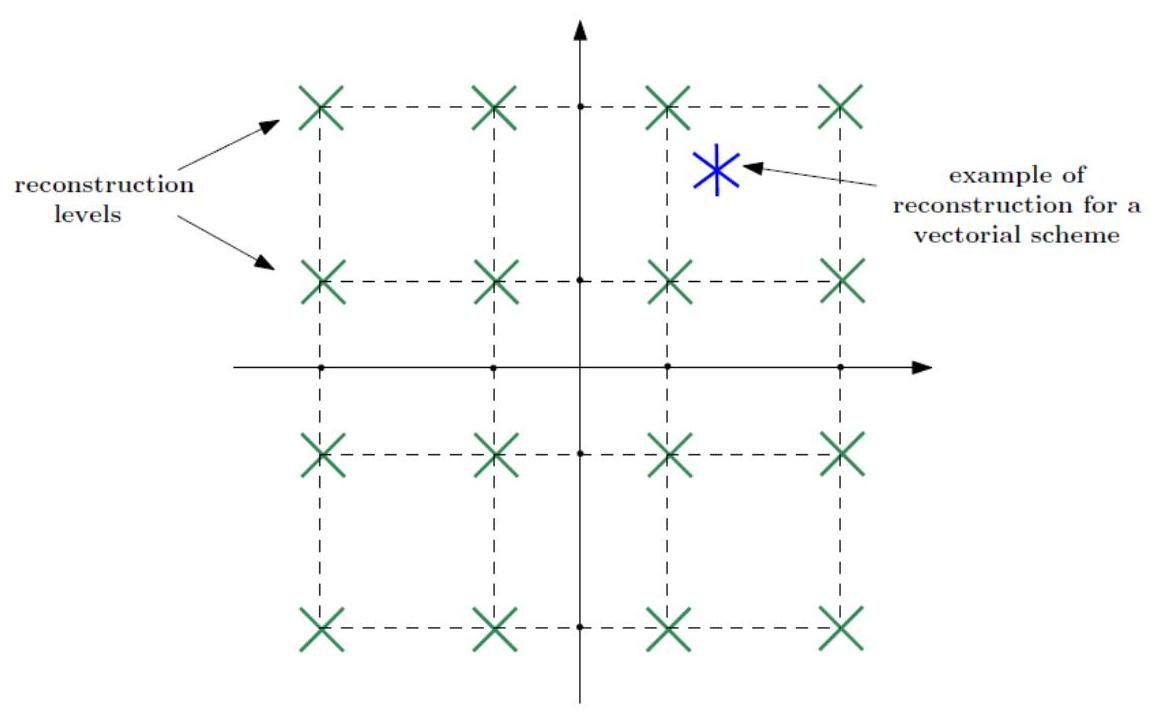
\includegraphics[scale=0.20]{img/ret.jpg}
    \caption{Quantizzazione a quadrati.}
    \label{fig:ret}
\end{figure}
\end{minipage} \hfill
\begin{minipage}{0.4\textwidth}
Con la quantizzazione vettoriale ci si svincola dalla forma quadrata delle celle: in questo caso, lavorando \textit{direttamente} in $\mathbb{R}^2$, il vettore quantizzato pu\`o assumere qualsiasi valore.
\begin{figure}[H]
    \centering
    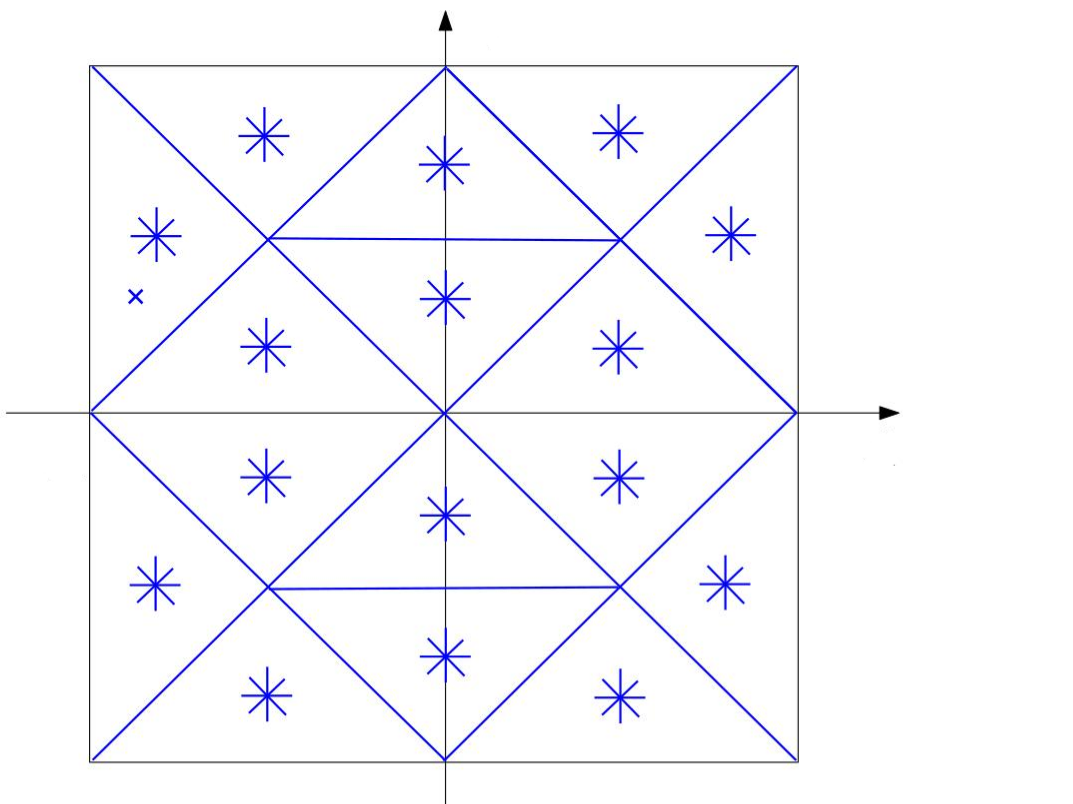
\includegraphics[scale=0.180]{img/vect.png}
    \caption{Tassellazione triangolare (esempio di quantizzazione vettoriale).}
    \label{fig:vect}
\end{figure}
\end{minipage} \\

Nella quantizzazione vettoriale c'\`e più libertà nella definizione delle regioni di quantizzazione perchè non si è vincolati ad una griglia rigida, come nel caso scalare. Anche nel caso di distribuzione uniforme con la quantizzazione vettoriale si riduce la distorsione. Si pu\`o mostrare che utilizzando, ad esempio, regioni esagonali
\begin{figure}[H]
    \centering
    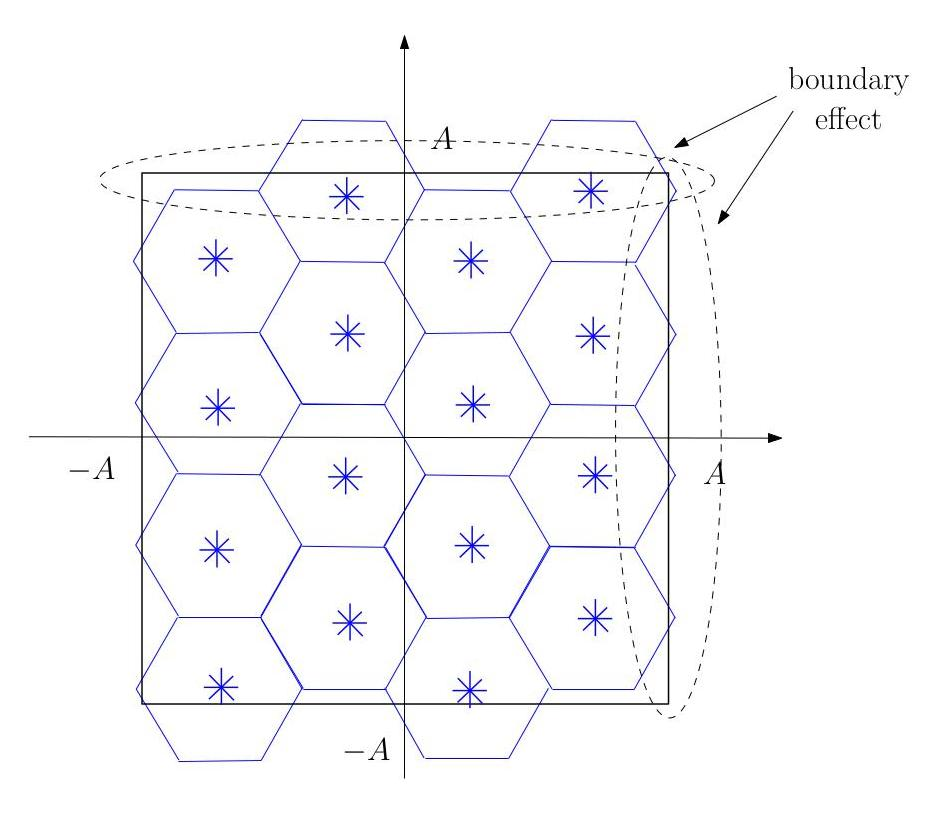
\includegraphics[scale=0.2]{img/hex.jpg}
    \caption{Tassellazione esagonale del dominio uniforme $[-A, A]^2$.}
    \label{fig:my_label}
\end{figure}
si pu\`o ridurre la distorsione. A parit\`a di area il calcolo dei momenti centrali d'inerzia suggerisce di utilizzare figure con pi\`u lati possibili, dovendoci avvicinare al minimo teorico dato dalla sfera. Questo induce per\`o dei problemi legati ad effetti di bordo, dati dal fatto che non \`e possibile ricoprire una regione quadrata con poligoni con pi\`u di 4 lati. Questo effetto diventa trascurabile all'aumentare del numero di intervalli di quantizzazione, ovvero eseguendo una \textit{quantizzazione fine}. 

\begin{mybox}{green}{\textit{\textbf{Esempio 2} : \textbf{Sorgenti con memoria. }}}
Nelle sorgenti con memoria, il beneficio è ancora più evidente: siano $X,Y$ due v.a. con pdf congiunta
\begin{equation}
    f_{XY}(x,y) = \begin{cases}
    \frac{1}{ab}, & (x,y) \in \mathcal{A}, \\
    0, & \text{ altrimenti.}
    \end{cases}
\end{equation}
dove $\mathcal{A}$ \`e la regione rettangolare delimitata da due lati $a$ e $b$ come in Figura \ref{fig:rett}:
\begin{figure}[H]
    \centering
    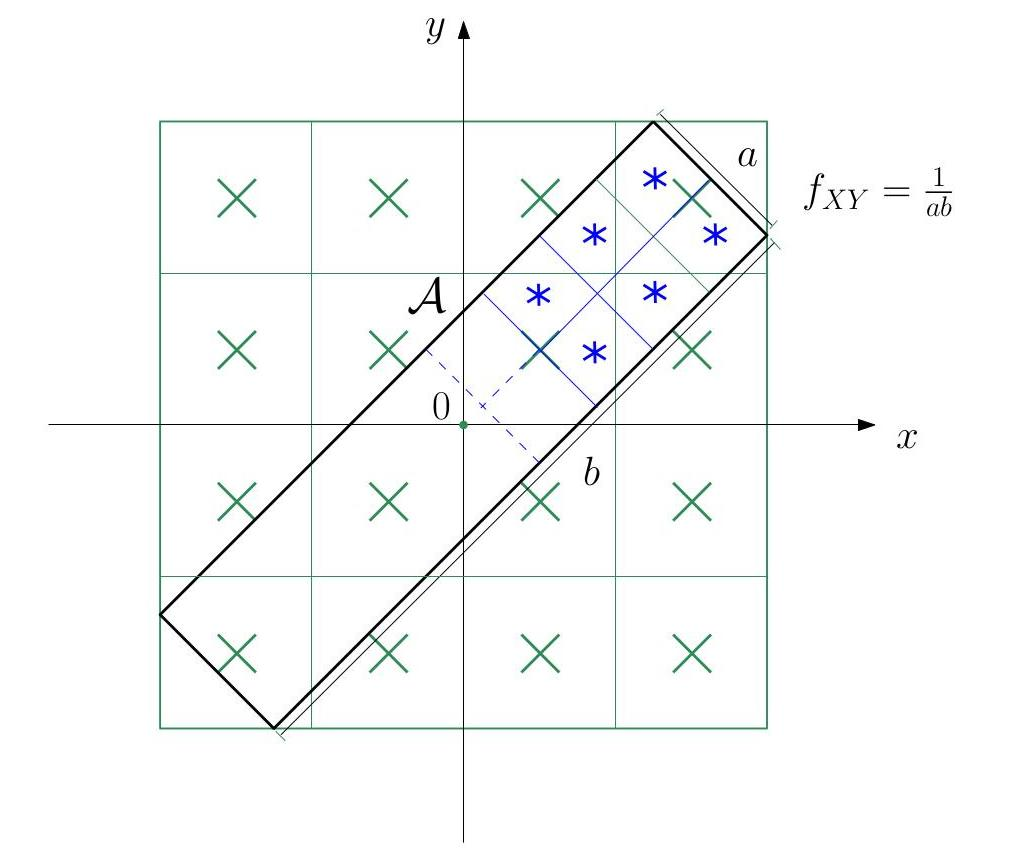
\includegraphics[scale=0.2]{img/rettang.jpg}
    \caption{Esempio di due v.a. correlate $X$ e $Y$. La quantizzazione vettoriale (stelline in blu) risulta necessaria dal momento che ogni struttura scalare (tassellazione in verde) porta ad una distribuzione non soddisfacente dei punti ricostruiti.}
    \label{fig:rett}
\end{figure}
Con la quantizzazione scalare si ottiene un risultato inefficiente dal momento che ci sono molte aree che non sono mai interessate dai valori, visto che questa tiene conto solo delle marginali $f_X(x), f_Y(y)$, non rendendo la quantizzazione efficiente dal punto di vista dello spreco di risorse. La correlazione tra $X$ e $Y$ rende necessario il dover ricorrere ad una quantizzazione vettoriale.
\end{mybox}